\documentclass{book}

\usepackage{graphicx}
\usepackage{wrapfig}
\usepackage{amsmath}

\graphicspath{{figure/out/}}

\title{Calcul pour NOCa}
\author{Yannis Benchaib--Langon}
\begin{document}
\maketitle

\section*{Introduction}
Ce document a pour but d'expliquer les calculs qui sont effectués dans la bibliothèque NOCa, aussi bien d'un point de vue physique que géométrique. Ce document présentera aussi les conventions utilisées dans cette bibliothèque.

\chapter*{Annexes géométriques}

\section*{L'Ellipse}


\begin{wrapfigure}{r}{0.4\textwidth}
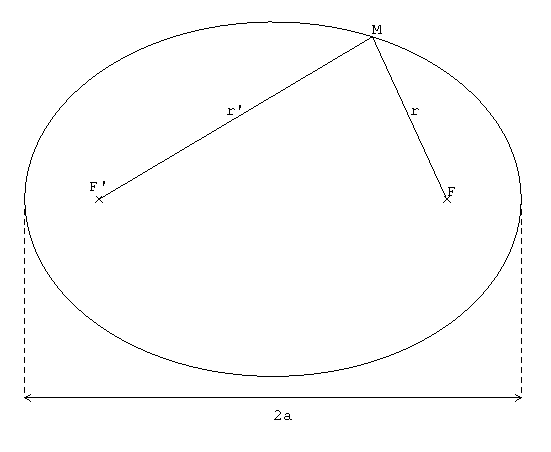
\includegraphics[width=0.9\linewidth]{A1_1.png}
\caption{exemple d'ellipse}
\end{wrapfigure}

Une ellipse est l'ensemble des points tel que la somme de la distance $r$ et $r'$ respectivement entre le point et le foyer $F$ et le point et le foyer $F'$ soit égal à la longueur du grand-axe : $2a$.

Autrement dit : 
\begin{equation}
\label{eq:A1.1}
r + r' = 2a
\tag{A1.1}
\end{equation}
Sur la figure ci-contre M appartient à l'ellipse tracée.
\\	Les deux foyers de l'ellipse sont espacés du distance de $2ae$

\subsection*{Équation cartésienne de l'ellipse}

L'ellipse définie comme au-dessus ne permet de la tracer faciliment car une équation comme (\ref{eq:A1.1}) est plus qu'implicite. On va alors trouver une forme cartésienne de cette équation.

\begin{wrapfigure}{l}{0.4\textwidth}
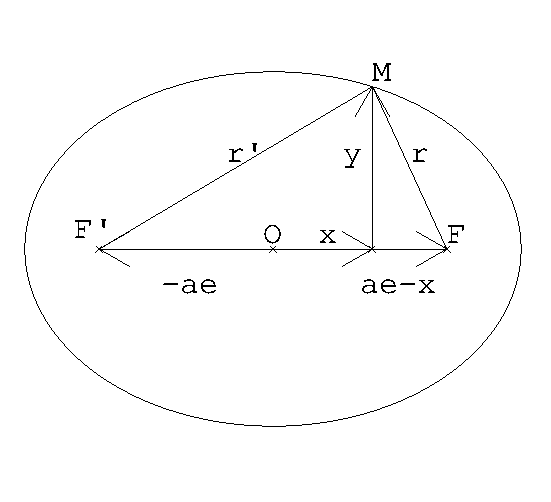
\includegraphics[width=0.9\linewidth]{A1_2.png}
\end{wrapfigure}

Sur la figure ci-contre, O sera notre origine et est placé au centre de l'ellipse c'est-à-dire au milieu des deux foyers. Ainsi, on définit x et y en fonction de O.\\
\begin{equation*}
r^2 = (ae-x)^2 + y^2 $$et$$ r'^2 = (x+ae)^2 + y^2
\end{equation*}

\begin{align*}
r+r'&=2a\\
r'&=2a-r\\
(ae+x)^2+y^2&=4a^2-4ar+(x-ae)^2+y^2\\
(ae)^2+2aex+x^2&=4a^2-4ar+x^2-2aex+(ae)^2\\
-4a(a-ex) &= -4ar\\
r&=a-ex\tag{A1.2}\\\label{eq:A1.2}
(x-ae)^2+y^2&=a^2-2aex+(ex)^2\\
x^2-2aex+(ae)^2+y^2-(ex)^2&=a^2-2aex\\
(1-e^2)x^2+y^2&=(1-e^2)a^2
\end{align*}

\begin{wrapfigure}{l}{0.4\textwidth}
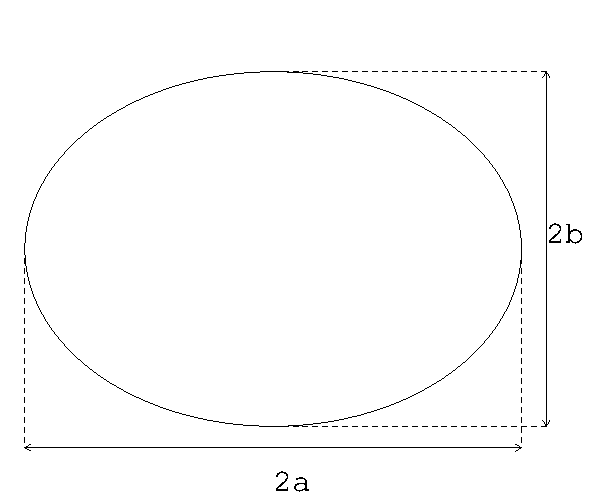
\includegraphics[width=0.9\linewidth]{A1_3.png}
\end{wrapfigure}

\begin{equation}
\label{eq:A1.3}
\boxed{\frac{x^2}{a^2}+\frac{y^2}{b^2}=1}
\tag{A1.3}
\end{equation}

où $b=a\sqrt{1-e^2}$ est la longueur du demi petit axe

\end{document}